\documentclass[dvipdfmx]{jarticle}
\usepackage{graphicx}
\usepackage[top=30truemm,bottom=30truemm,left=25truemm,right=25truemm]{geometry}
\usepackage{listings,jvlisting}

\lstset{
  basicstyle={\ttfamily},
  identifierstyle={\small},
  commentstyle={\smallitshape},
  keywordstyle={\small\bfseries},
  ndkeywordstyle={\small},
  stringstyle={\small\ttfamily},
  frame={tb},
  breaklines=true,
  columns=[l]{fullflexible},
  numbers=left,
  xrightmargin=0zw,
  xleftmargin=3zw,
  numberstyle={\scriptsize},
  stepnumber=1,
  numbersep=1zw,
  lineskip=-0.5ex
}

\begin{document}
\begin{titlepage}
    \begin{center}
        {\huge 情報科学演習C 課題4レポ―ト}
        \vspace{180pt}\\
        \begin{tabular}{rl}
            氏名 & 山久保孝亮\\
            所属 & 大阪大学基礎工学部情報科学科ソフトウェア科学コース\\
            メールアドレス & u327468b@ecs.osaka-u.ac.jp\\
            学籍番号 & 09B22084\\
            提出日 & \today\\
            担当教員 & 平井健士,中島悠太
        \end{tabular}
    \end{center}
\end{titlepage}
\section{課題4-1}
\subsection{プログラムの仕様}
課題4-1で作成したクライアントプログラムchatclient.cの仕様は以下の通りである.
\begin{itemize}
    \item プログラム実行の書式は"./chatclient [サーバプログラムを実行中のホスト名] [使用したいユーザ名]"である.
    \item 接続できたかどうか,名前を登録できたかどうかが標準出力に表示される.接続できた場合はチャット機能が使用でき,接続できなかった場合はプログラムが終了する.
    \item チャット機能には以下の3つの機能がある.
    \begin{enumerate}
        \item 標準入力に文字列を書き込んで[Enter]キーを押すと,サーバにその文字列を送信する.
        \item サーバに接続されているほかのホストから送られてきた文字列を受信し,標準入力に表示させる.
        \item EOFを入力するとサーバとの接続が切れ,プログラムを終了する.
    \end{enumerate}
\end{itemize}
また,サーバプログラムchatserver.cの仕様は以下の通りである.
\begin{itemize}
    \item プログラム実行の書式は引数はなしである.即ち"./chatserver"である.
    \item 一度に接続できるユーザの数は5つである.
    \item 常に新たなユーザの接続を待っており,新たに接続しようとするユーザが現れた場合には正常に接続できたかどうかと,すでに同じユーザ名が登録されていないかを確認する.どちらも
    満たしていればその旨の文字列を送信して新たなユーザとして登録し,いずれかを満たさない場合はその旨の文字列を送信して再び待ち状態に入る.
    \item 登録されたユーザから文字列を受信した場合は,その文字列の先頭にユーザ名を追加して接続中のすべてのクライアントに送信する.
    \item EOFを受信するとそのユーザの接続を切り,ユーザの情報を削除する.
\end{itemize}
また,両社のプログラムに共通する仕様は以下のとおりである.
\begin{itemize}
    \item 使用するポート番号は10140である.
    \item ユーザ名は英数字,ハイフン,アンダースコアのみから成る.
    \item クライアント側はユーザ名の末尾に改行文字を追加して送信し,サーバ側は受け取った際にその改行文字を取り除いてから保存する.
\end{itemize}
\subsection{クライアントプログラムのアルゴリズム}
今回作成したプログラムは指導書の状態に則って作成しており,以下の図1のフローチャートはそれぞれの状態の遷移の様子を表す.
\clearpage
\begin{figure}[h]
    \centering
    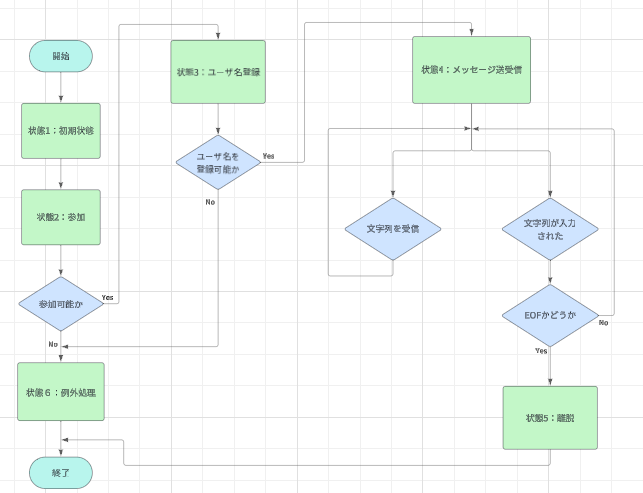
\includegraphics[width=10cm]{4-1clienthurotya.png}
    \caption{クライアントプログラムのフローチャート}
\end{figure}
それぞれの状態は指導書のとおりに実装した.また,図1には現れていないが状態6の例外処理はプログラム中の操作に問題が発生した際に実行されるので,任意の状態から状態6に遷移する.それぞれの状態の概要は以下のとおりである.
\begin{description}
    \item[状態1:初期状態]  \\  ソケットを作成し,第一引数のホスト名に接続要求を出す.
    \item[状態2:参加] \\ サーバから接続できたかどうかの文字列を受け取り,判定する.
    \item[状態3:ユーザ名登録] \\ 第二引数のユーザ名を送信し,ユーザ名を登録できたかどうかの文字列を受け取る.そしてそれを判定する.
    \item[状態4:メッセージ送受信] \\ 標準入力から文字列が入力されればその文字列をサーバへ送信する.サーバから文字列を受信すればその文字列を標準入力へ出力する.
    \item[状態5:離脱] \\ 標準入力が"EOF"のとき,ソケットを閉じてプログラムを正常終了する.
    \item[状態6:例外処理] \\ 何らかの操作においてエラーが発生した際に,ソケットを閉じてプログラムを異常終了する.
\end{description}
\subsection{クライアントプログラムの実装方法}
ここではアルゴリズムで記述した各状態とその条件分岐の詳細な実装方法について記述する.
以下の表1はこのプログラムで使用した変数名とその表す内容である.
\clearpage
\begin{table}[h]
    \centering
    \begin{tabular}{|c|c|c|}
        \hline
        変数名 & 型 & 表す内容\\\hline\hline
        sock & int & ソケットディスクリプタ\\\hline
        n & int & 入出力操作の結果を格納\\\hline
        rbuf & char & 送受信する文字列を格納する.要素数は1024\\\hline
        rfds & fd\_set & ファイルディスクリプタのセット\\\hline
        tv & struct timeval & タイムアウト値を設定する構造体\\\hline
        *server & struct hostent & ホスト情報を格納するためのポインタ\\\hline
        svr & struct sockaddr\_in & サーバのアドレス情報を格納する構造体\\\hline
        current\_time & time\_t & 現在の時刻を格納\\\hline
        *local\_time & struct tm & ローカルタイムを表す構造体へのポインタ\\\hline
        argc & int & 引数の個数を格納\\\hline
        *argv[] & char & 引数の文字列を格納\\\hline
    \end{tabular}
    \caption{このプログラムで使用した変数}
\end{table}
\subsubsection{初期状態}
状態1のプログラムは大きく以下のように処理が分かれる.
\begin{enumerate}
    \item 書式の確認し,ソケットを作成
    \item ホスト名を取得し,接続する
\end{enumerate}
以下でその詳細について記述する.
\begin{enumerate}
    \item この処理のプログラムは以下のようになる.
\begin{lstlisting}
if(argc != 3){
    fprintf(stderr, "Usage: %s <hostname> <username>\n", argv[0]);
    exit(1);
}
if ((sock=socket(AF_INET,SOCK_STREAM,IPPROTO_TCP))<0) {
    perror("socket");
    exit(1);
}
\end{lstlisting}
コマンドライン引数が3であるかどうかを確認して書式が正しいかを確認する.ここでargcの値が3である理由は"./chatclient"も引数として数えられるためである.
そしてsock()を使ってソケットを作成する.
    \item この処理のプログラムは以下のようになる.
\begin{lstlisting}
server = gethostbyname(argv[1]);
if (server == NULL) {
    fprintf(stderr, "ERROR, no such host as %s\n", argv[1]);
    exit(0);
}
bzero((char *)&svr, sizeof(svr));
svr.sin_family = AF_INET;
bcopy((char *)server->h_addr, (char *)&svr.sin_addr.s_addr, server->h_length);
svr.sin_port = htons(10140);
if (connect(sock, (struct sockaddr *)&svr, sizeof(svr)) < 0) {
状態6の処理
}
\end{lstlisting}
コマンドライン引数の1番目の引数をホスト名として変数に格納する.ここでインデックスが1である理由はargv[0]に"./chatclient"が格納されているからである.
そしてそのホスト名のサーバがあればconnect()を使って接続をサーバに要請する.
\end{enumerate}
\subsubsection{参加}
状態2のプログラムは以下のようになる.
\begin{lstlisting}
bzero(rbuf, 1024);
n = read(sock, rbuf, 1024);
if(n <= 0){
状態6の処理
}
printf("%s",rbuf);
if(strcmp(rbuf,"REQUEST ACCEPTED\n") == 0) {
状態3の処理
}else{
状態6の処理}
\end{lstlisting}
まずサーバから文字列を受信しそれを標準入力に出力する.正常に受信ができればその内容が"REQUEST ACCEPTED \textbackslash n"であるので,一致しているかどうかを確認し一致していれば状態3へ,一致していなければ状態6へ遷移する.
文字列が一致しているかどうかの判定にはstrcmp()を使用した.
\subsubsection{ユーザ名登録}
状態3のプログラムは大きく以下のように処理が分かれる.
\begin{enumerate}
    \item ユーザ名を処理してからサーバへ送信する.
    \item サーバからユーザ名の登録に関する文字列を受け取る.
\end{enumerate}
以下でその詳細について記述する.
\begin{enumerate}
    \item この部分の処理のプログラムは以下のようになる.
    \begin{lstlisting}
bzero(rbuf,1024);
strcpy(rbuf,argv[2]);
rbuf[strlen(argv[2])] = '\n';
n = write(sock, argv[2], strlen(argv[2]));
if(n < 0){
    状態6の処理
}
    \end{lstlisting}
    まず第二引数のユーザ名をサーバに送信する.
    引数を送信する際,ユーザ名の終わりを判別するために改行文字を最後に加える.また,rbufをbzero()を使って初期化してからユーザ名を格納している.
    これをしていないと,例えば"aiueo"というユーザ名にした場合rbufに格納されている文字列が"aiueoST ACCEPED\textbackslash n"という文字列になってしまうので
    前の文字列を初期化しなければならない.
    \item この部分の処理のプログラムは以下のようになる.
    \begin{lstlisting}
bzero(rbuf, 1024);
n = read(sock, rbuf, 1024);
if(n <= 0){
    状態6の処理
}
printf("%s",rbuf);  
    \end{lstlisting}
    この処理でもbzero()でrbufを初期化してからread()を使って文字列を受け取っている.
\end{enumerate}
\subsubsection{メッセージ送受信}
状態4と待ち状態のプログラムは大きく以下のように処理が分かれる.
\begin{enumerate}
    \item 待ち状態によるソケットと標準入力の監視
    \item 送信処理
    \item 受信処理
\end{enumerate}
以下でその詳細について記述する.
\begin{enumerate}
    \item この処理のプログラムは以下のようになる.
    \begin{lstlisting}
while(1){
    FD_ZERO(&rfds);
    FD_SET(0, &rfds);
    FD_SET(sock, &rfds);
    tv.tv_sec = 1;
    tv.tv_usec = 0;
    if (select(sock + 1, &rfds, NULL, NULL, &tv) > 0) {
        if (FD_ISSET(0, &rfds)) {
            送信      
        }
        if (FD_ISSET(sock, &rfds)) {
            受信
        }
    }
} 
    \end{lstlisting}
    while文による無限ループの中でselect()を使って標準入力とソケットを監視している.FD\_ISETの第一引数が0であれば送信,sockであれば
    受信の処理へ移る.
    \item この処理のプログラムは以下のようになる.
    \begin{lstlisting}
bzero(rbuf, 1024);
if (fgets(rbuf, 1024, stdin) == NULL) {
    状態5の処理
}
n = write(sock, rbuf, strlen(rbuf));
if (n < 0) {
    状態6の処理
}
    \end{lstlisting}
    ここではwrite()を使ってメッセージの送信の処理を実装している.fgets()によって標準入力から取得された文字列をrbufへ格納して送信している.このとき,EOFが入力された時は状態5に遷移する.
    \item この処理のプログラムは以下のようになる.
    \begin{lstlisting}
bzero(rbuf, 1024);
n = read(sock, rbuf, 1024);
if(n <= 0){
    状態6の処理
}else{
    printf("%s",rbuf);
}
    \end{lstlisting}
\end{enumerate}
\subsubsection{離脱}
状態5のプログラムは以下のようになる.
\begin{lstlisting}
printf("\nEOF detected\n");
close(sock);
exit(0);
\end{lstlisting}
EOFが入力されたことを表示し,ソケットを閉じてexit(0)でプログラムを正常終了する.
\subsubsection{例外処理}
状態6のプログラムは以下のようになる.
\begin{lstlisting}
perror("ERROR MESSAGE");
close(sock);
exit(1);
\end{lstlisting}
この状態は何らかの処理が正常に動作しなかった際の処理のため,まずperror()を使ってそれぞれの問題に合わせたエラーメッセージを表示する.そしてソケットを閉じてexit(1)でプログラムを異常終了する.
\subsection{サーバプログラムのアルゴリズム}
今回作成したプログラムは指導書の状態に則って作成しており, 以下の図2のフローチャートはそれぞれ
の状態の遷移の様子を表す.
\clearpage
\begin{figure}[h]
    \centering
    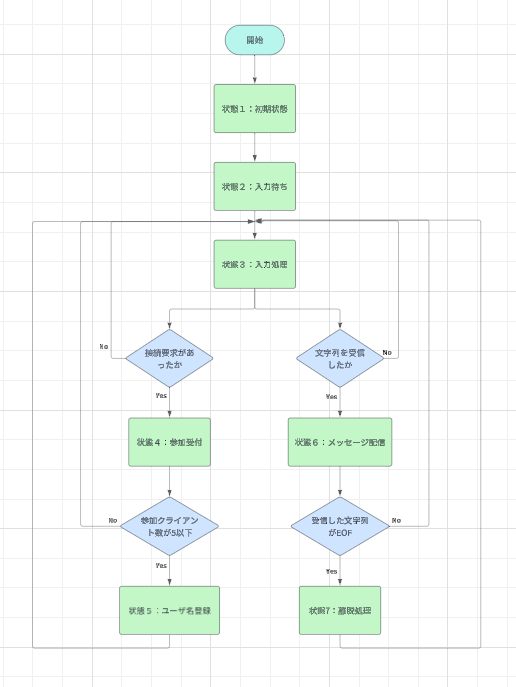
\includegraphics[width=8cm]{4-1serverhurotya.png}
    \caption{クライアントプログラムのフローチャート}
\end{figure}
それぞれの状態は指導書のとおりに実装した.また,図2には現れていないが状態7の例外処理はプログラム中の操作に問題が発生した際に実行されるので,任意の状態から状態7に遷移する.それぞれの状態の概要は以下のとおりである.
\begin{description}
    \item[状態1:初期状態]  \\  ソケットを作成し,バインドする.
    \item[状態2:入力待ち] \\ 接続要求とクライアントからの文字列の受信を監視する.
    \item[状態3:入力処理] \\ 接続要求があった場合とクライアントからの文字列の受信があった場合で処理を分岐させる.
    \item[状態4:参加受付] \\ 接続要求を受け付け,待ち受け可能数を超えていなければ登録完了メッセージを送信する.超えている場合は接続拒否のメッセージを送信する.
    \item[状態5:ユーザ名登録] \\ ユーザ名を受信し,現在接続中のクライアントと同じ名前でなければ登録完了メッセージを送信する.同じ名前があれば登録拒否メッセージを送信する.
    \item[状態6:メッセージ配信] \\ 受信した文字列の先頭にユーザ名を追加して接続中の全クライアントに対してその文字列を送信する.
    \item[状態7:離脱処理] \\ 何らかの操作においてエラーが発生した際に,ソケットを閉じてプログラムを異常終了する.
\end{description}
\subsection{サーバプログラムの実装方法}
ここではアルゴリズムで記述した各状態とその条件分岐の詳細な実装方法について記述する.
以下の表2はこのプログラムで使用した変数名とその表す内容である.
\begin{table}[h]
    \centering
    \begin{tabular}{|c|c|c|}
        \hline
        変数名 & 型 & 表す内容\\\hline\hline
        sock & int & ソケットディスクリプタ\\\hline
        n & int & 入出力操作の結果を格納\\\hline
        k & int & 現在接続されているクライアントの個数を格納\\\hline
        sd & int & クライアントソケットのファイルディスクリプタ\\\hline
        clen & int & クライアントアドレスのアドレス構造体のサイズを格納\\\hline
        max\_sd & int & select()で使用するファイルディスクリプタの最大値を格納\\\hline
        new\_socket & int & 新しいクライアント接続のためのソケットファイルディスクリプタ\\\hline
        new\_socket\_num & int & 新しく接続されたクライアントのソケット番号を格納\\\hline
        username\_flag & int & ユーザ名の重複を確認するためのフラグ.\\\hline
        csock & int & 接続されたクライアントのファイルディスクリプタを格納する配列\\\hline
        registered\_username & char & 登録されたユーザ名を格納する配列\\\hline
        svr & struct sockaddr\_in & サーバのアドレス情報を格納する構造体\\\hline
        clt & struct sockaddr\_in & サーバのアドレス情報を格納する構造体\\\hline
        rfds & fd\_set & ファイルディスクリプタのセット\\\hline
        tv & struct timeval & タイムアウト値を設定する構造体\\\hline
        rbuf & char & 送受信する文字列を格納する.要素数は1024\\\hline
        name\_message & char & メッセージを構築するためのバッファ\\\hline
        accept\_request\_message & char & "REQUEST ACCEPTED \textbackslash n"を格納\\\hline
        reject\_request\_message & char & "REQUEST REJECTED \textbackslash n"を格納\\\hline
        accept\_username\_message & char & "USERNAME ACCEPTED \textbackslash n"を格納\\\hline
        reject\_username\_message & char & "USERNAME REJECTED \textbackslash n"を格納\\\hline
    \end{tabular}
    \caption{このプログラムで使用した変数}
\end{table}
\subsubsection{初期状態}
状態1のプログラムは大きく以下のように処理が分かれる.
\begin{enumerate}
    \item 配列csockを全て-1に初期化
    \item 接続のための設定
\end{enumerate}
以下でその詳細について記述する.
\begin{enumerate}
    \item この処理のプログラムは以下のようになる.
    \begin{lstlisting}
for (int i = 0; i < MAXCLIENTS; i++) {
    csock[i] = -1;
    bzero(registered_username[i],256);
} 
    \end{lstlisting}
    ここではfor文によりクライアントのファイルディスクリプタを格納するための配列であるcsockの全要素を-1に初期化している.これにより,-1が格納されていればそのインデックスには
    クライアントは接続されておらず,-1以外であればクライアントが接続されていると見分けることができる.
    \item この処理のプログラムは以下のようになる.
    \begin{lstlisting}
if ((sock=socket(AF_INET,SOCK_STREAM,IPPROTO_TCP))<0) {
    perror("socket");
    exit(1);
}
bzero(&svr,sizeof(svr));
svr.sin_family=AF_INET;
svr.sin_addr.s_addr=htonl(INADDR_ANY);
svr.sin_port=htons(10140);
if(bind(sock,(struct sockaddr *)&svr,sizeof(svr))<0) {
    perror("bind");
    exit(1);
}
if (listen(sock,5)<0) {
    perror("listen");
    exit(1);
}
k=0;
    \end{lstlisting}
    まずsocket()でソケットを作成し,bind()でsockに待ち受けするネットワークインターフェイスを割り当てる.そして現在接続されているクライアント数を表すkを0に初期化する.
\end{enumerate}
\subsubsection{入力待ち}
状態2のプログラムは以下のようになる.
\begin{lstlisting}
while(1){
    FD_ZERO(&rfds);
    FD_SET(0, &rfds);
    FD_SET(sock, &rfds);
    tv.tv_sec = 1;
    tv.tv_usec = 0;
    max_sd = sock;
    for(int i=0;i<MAXCLIENTS;i++){
        sd = csock[i];
        if(sd > 0){
            FD_SET(sd, &rfds);
        }
        if (sd > max_sd) {
            max_sd = sd;
        }
    }
    if (select(max_sd + 1, &rfds, NULL, NULL, &tv) > 0) {
        状態3の処理
    }            
}
\end{lstlisting}
ここでは無限ループの中にselect()を使用するための初期化の処理を記述する.また,8行目からのfor文ではcsockの内,ソケットディスクリプタが格納されているインデックスを探してそれと現在のmax\_sdを比較して最大のソケットディスクリプタを格納できるようにしている.
そしてselect()を実行する.
\subsubsection{入力処理}
状態3のプログラムは以下のようになる.
\begin{lstlisting}
if (FD_ISSET(sock, &rfds)) {
    状態4の処理        
}
for(int i=0;i<MAXCLIENTS;i++){
    if ((csock[i] != -1) && (FD_ISSET(csock[i], &rfds))){
        状態6の処理
    }
}
\end{lstlisting}
1から3行目では接続要求があるかどうかをFD\_ISSET()を使って監視している.また,4から8行目では,csockに格納されている登録済みのクライアントからのメッセージの受信を監視している.
\subsubsection{参加受付}
状態4のプログラムは以下のようになる.
\begin{lstlisting}
clen = sizeof(clt);
if ((new_socket = accept(sock, (struct sockaddr *)&clt, &clen)) < 0) {
    perror("accept");
    exit(2);
}
if(k<MAXCLIENTS){
    n = write(new_socket, accept_request_message, strlen(accept_request_message));
    if(n < 0){
        perror("ERROR writing");
        close(new_socket);
        break;
    }
    状態5の処理
}else{
    n = write(new_socket, reject_request_message, strlen(reject_request_message));
    if(n < 0){
        perror("ERROR writing");
        close(new_socket);
        break;
    }
    close(new_socket);
}
\end{lstlisting}
1から5行目ではaccept()を使ってクライアントからのconnect()による接続要求を受け入れている.6から19行目の条件分岐では,
現在接続中のクライアントの個数kが5より小さいとき,即ちまだクライアントを接続できるときの処理である.このとき,write()で接続が受け入れられた旨の文字列を送信する.12行目から18行目の条件分岐では
kが5以上,即ちこれ以上クライアントを接続することができないときに実行される.このときwrite()を使って接続が受け入れられなかった旨の文字列を送信し,2行目で受け入れたnew\_socketを閉じている.
\subsubsection{ユーザ名登録}
状態5のプログラムの処理は大きく以下のように分けることができる.
\begin{enumerate}
    \item 登録可能なソケット番号を確認し,登録するユーザ名を取得
    \item ユーザ名に関する処理
    \item 登録するユーザ名が既に登録されていないかの確認
    \item フラグによる分岐とそれぞれの処理
\end{enumerate}
以下でその詳細について記述する.
\begin{enumerate}
    \item この部分の処理のプログラムは以下のようになる.
    \begin{lstlisting}
for (int i = 0; i < MAXCLIENTS; i++) {
    登録可能なソケット番号を確認
    if (csock[i] == -1) {
        new_socket_num = i;
        csock[i] = new_socket;
        break;
    }
}
bzero(rbuf, 1024);
n = read(new_socket, rbuf, 1024);
登録するユーザー名を取得
if(n <= 0){
    perror("Connection closed by client.\n");
    close(new_socket);
    return 0;
}
    \end{lstlisting}
    1から8行目までのfor文ではcsockのそれぞれの要素が-1であるか,即ち登録可能な要素が残っているかを調べている.まだ登録可能なものが残っていればnew\_socket\_numにそのインデックスを
    格納し,csockのそのインデックス番目の要素にソケットディスクリプタを格納しbreakする.これにより,一つ登録可能な要素が見つかればこのfor文は終了する.

    9から16行目ではrbufをbzero()で初期化してからread()でクライアントから送信されるユーザ名を取得している.
    \item この部分の処理のプログラムは以下のようになる.
    \begin{lstlisting}
username_flag = 0;
for(int i=0;i<1024;i++){
    if(rbuf[i] == '\n'){
        rbuf[i] = '\0';
        break;
    }
    if(!isalnum(rbuf[i]) && rbuf[i] != '_' && rbuf[i] != '_'){
        username_flag = 1;
    }
}
    \end{lstlisting}
    1行目のusername\_flagはユーザ名を受け付けるか拒否するかを表すフラグであり,0は拒否を,1は受け付けることを表す.2から10行目のfor文では,受信したユーザ名の末尾から改行文字"\textbackslash n"を取り除き,ユーザ名に英数字とハイフン,アンダーバー以外の文字が含まれていないかを判定している.
    改行文字の除去は3から6行目のように文字列の要素を"\textbackslash n"を比較し一致していればそれをヌル文字に変換することで実現した.
    指定された文字以外が含まれていないかの判定は7から9行目のように指定された3つの条件全てを満たさないものがあればフラグを1にすることで実現した.フラグについての処理は後述する.

    また,仕様よりユーザ名は英数字とハイフン,アンダースコアのみから成るのでユーザ名の途中に改行文字が存在し,正確に処理されないということはあり得ない.
    \item この部分の処理のプログラムは以下のようになる.
    \begin{lstlisting}
for(int i=0;i<MAXCLIENTS;i++){
    if (strcmp(registered_username[i], rbuf) == 0) {
        username_flag = 1;
        break;
    }
}
    \end{lstlisting}
    for文を使って登録されたユーザ名を格納しているregisted\_usernameの全要素と今回新たに受信したユーザ名とを比較し,一致しているものがないかをstrcmp()を使って判定する.
    同じであればフラグを1にしてbreakする.
    \item この部分の処理のプログラムは以下のようになる.
    \begin{lstlisting}
if(username_flag == 0){
    n = write(new_socket, accept_username_message, strlen(accept_username_message));
    if(n < 0){
        perror("ERROR writing");
        close(new_socket);
        break;
    }
    strcpy(registered_username[new_socket_num], rbuf);
    printf("%s is registered\n",registered_username[new_socket_num]);
    csock[new_socket_num] = new_socket;
    k++;
}else{
    n = write(new_socket, reject_username_message, strlen(reject_username_message));
    if(n < 0){
        perror("ERROR writing");
        close(new_socket);
        break;
    }
    csock[new_socket_num] = -1;
    close(new_socket);
}
        \end{lstlisting}
        1から12行目の条件分岐はフラグが0,即ちユーザ名が登録可能であるときの処理である.ユーザ名の登録を受け付けた旨の文字列をwrite()で送信しregistered\_usernameのnew\_socket\_num番目の要素に
        strcpy()を使ってユーザ名を格納する.また,csockのnew\_socket\_num番目に新たに登録するソケットディスクリプタnew\_socketを格納する.これにより,registered\_usernameとcsockのインデックスはそれぞれ対応する.
        そして最後に接続しているクライアント数を1つインクリメントする.

        12行目から21行目の条件分岐ではフラグが1,即ちユーザ名が登録可能ではないときの処理である.ユーザ名の登録を拒否した旨の文字列をwrite()で送信し,csockのnew\_socket\_num番目の要素を-1に,new\_socketを閉じる.
    \end{enumerate}

\subsubsection{メッセージ配信}
状態6のプログラムは以下のようになる.
\begin{lstlisting}
bzero(rbuf, 1024);
n = read(csock[i], rbuf, 1024);
if(n <= 0){
    状態7の処理
}else{
    for(int j=0;j<MAXCLIENTS;j++){
        if(csock[j] != -1){
            snprintf(name_message, sizeof(name_message), ">%s %s", registered_username[i], rbuf);
            n = write(csock[j], name_message, strlen(name_message));
            if(n < 0){
                perror("ERROR writing");
                break;
            }
        }
    }
}
\end{lstlisting}
このプログラムはcsockのすべての要素の内のいずれか一つから文字列を受信すると実行される.即ち,このプログラムが処理されるのはcsock[i]から文字列を受信したときである.
まずクライアントcsock[i]から送信された文字列をread()で受け取る.3から5行目の処理はクライアントがEOFを入力したときの処理である.
5から16行目はEOF以外の文字列が入力された時の処理である.ここでは受け取った文字列を接続中のクライアントすべてに送信している.
具体的には6から15行目のfor文の中で以下の処理を実行する.
\begin{itemize}
    \item csockの値が-1かどうかを判定して,接続中のインデックスのみに以下の処理を実行する.
    \item snprintf()を使って先頭に">[ユーザ名] [送信する文字列]"をname\_messageに格納する.ユーザ名はregistered\_username[i]に格納されている.
    \item write()を使ってname\_messageを送信する.
\end{itemize}
\subsubsection{離脱処理}
状態7のプログラムは以下のようになる.
\begin{lstlisting}
close(csock[i]);
printf("%s has left the chat room\n",registered_username[i]);
k--;
csock[i] = -1;
bzero(registered_username[i],256);
break;
\end{lstlisting}
まずcsock[i]を閉じ,i番目のクライアントが退出した旨のメッセージを標準入力に出力する.次に接続中のクライアント数kを一つ減らし,csock[i]を-1に初期化する.また,registerd\_username[i]もbzero()で初期化する.
以上により,クライアントに関するすべての情報を初期化したのでbreakして再びselect()による待ち状態に戻る.
\subsection{実行結果}
今回の課題4-1の実行結果は以下のような場合に分類することができる.
\begin{enumerate}
    \item 一人だけ適切なユーザ名で接続された時\\
    あ
    \item 二人だけ適切なユーザ名で接続された時\\
    あ
    \item 五人だけ適切なユーザ名で接続された時\\
    \item 3の状態で新たに適切なユーザ名で接続された時\\
    \item 
\end{enumerate}
\section{課題4-2}
\subsection{プログラムの仕様}
\subsection{アルゴリズム}
\subsection{実装方法}
\subsection{実行結果}
\section{考察}
\section{感想}
\section{謝辞}
\end{document}